\documentclass[a4paper,12pt]{article}
\usepackage{float}
\usepackage[table]{xcolor} % Para colorir as linhas da tabela
\usepackage{array} % Para melhorar a formatação de tabelas
\usepackage[brazil]{babel}
\usepackage[utf8]{inputenc}
\usepackage{indentfirst}
\usepackage{amsmath}
\usepackage{multicol}
\usepackage{graphicx}
\usepackage{animate}
\usepackage{tabularx}
\usepackage[font=footnotesize, labelfont=bf, listformat=empty]{caption}
\usepackage{geometry}
\usepackage{listings}
\usepackage{lastpage}
\usepackage{subcaption}
\usepackage[skins,xparse,breakable]{tcolorbox}
\usepackage{longtable}
\usepackage{minted}
\usepackage{titlesec}
\usepackage{fancyhdr}
\usepackage{setspace}
\usepackage[colorlinks=true, allcolors=black]{hyperref}

% Configurações de margens e espaçamento
\geometry{a4paper, left=2.5cm, right=2.5cm, top=2.5cm, bottom=2cm}
\onehalfspacing

% Configurações de títulos
\titleformat{\section}{\normalfont\large\bfseries}{\thesection}{1em}{}
\titleformat{\subsection}{\normalfont\bfseries}{\thesubsection}{1em}{}
\titleformat{\subsubsection}{\normalfont\itshape}{\thesubsubsection}{1em}{}

% Configurações de listagens
\renewcommand{\listingscaption}{Código}
\newenvironment{code}{\captionsetup{type=listing}}{}

% Configurações de cores
\definecolor{LightSeaGreen}{rgb}{0.1255, 0.6980, 0.6667}
\definecolor{whitesmoke}{rgb}{0.96, 0.96, 0.96}
\definecolor{cinza}{RGB}{160, 160, 160}
\definecolor{cinza_claro}{RGB}{240, 240, 240} % Cinza claro

% Configurações do minted para VHDL
\setminted[VHDL]{
    fontsize=\footnotesize,
    style=emacs,
    linenos=true,
    breaklines=true,
    mathescape=true,
    bgcolor=cinza_claro,
    breakanywhere=true,
}

\newcommand{\hex}[1]{\textcolor{green!50!black}{#1}}

% Configurações de cabeçalho e rodapé
\pagestyle{fancy}
\fancyhf{}
\fancyhead[L]{\footnotesize{Laboratório de Sistemas Digitais - ENE0040}}
\fancyhead[R]{\footnotesize{2025/1 - Turma 07}}
\fancyfoot[R]{\footnotesize{Página \hspace{0.05cm} \thepage \hspace{0.05cm} de \pageref{LastPage}}}
\fancyfoot[L]{\footnotesize{Relatório do Experimento 5}}

% Adiciona uma linha preta acima do rodapé
\renewcommand{\footrulewidth}{0.4pt} % Espessura da linha
\renewcommand{\footrule}{\vbox to 0pt{\hrule width \textwidth height \footrulewidth \vss}} % Desenha a linha

% Novo Comando para chamar a capa
\newcommand{\capa}{
    \begin{titlepage}
        \begin{multicols}{2}
            \begin{flushleft}
                
\includegraphics[width=0.45\linewidth]{Recursos/Imagens/UnB_logo.png}
            \end{flushleft}
            \columnbreak
            \begin{flushright}
                Universidade de Brasília \\
                Faculdade de Tecnologia \\
                Departamento de Engenharia Elétrica
            \end{flushright}
        \end{multicols}
        \begin{center}
        \vspace{-20pt}
        \rule{\textwidth}{0.4pt}
        \end{center}
        \vspace{0.6cm}
        \begin{center}
            {\Huge \textbf{Relatório do Experimento 5}} \\[1em]
            {\large \textbf{Autor:} Henrique Morcelles Salum} \\[0.5em]
            {\large \textbf{Matrícula:} 232003008} \\
            \vfill
            {\large \textbf{ENE0040 - Laboratório de Sistemas Digitais - Turma 07}} \\
        \end{center}
    \end{titlepage}
}

\begin{document}

\capa

% Sumário
\newpage
\tableofcontents
\newpage

% Introdução
\section{Introdução}

\subsection{Sobre o Experimento}
Este experimento é separado em três tarefas, mas podemos tratá-las como apenas uma, pois todas são profundamente interligadas. Em suma, projetaremos um somador de 4 bits (\textit{nibble}), seu \textit{testbench} e um \textit{Golden Model}, para analisar os resultados obtidos. Tudo será projetado em VHDL e simulado no ModelSim.

O somador de \textit{nibble} tem dois vetores de entrada $A$ e $B$, de quatro \textit{bits} e um vetor de saída $S$, de cinco \textit{bits}. O circuito principal é implementado por meio de instâncias de somadores completos; o \textit{Golden Model} é implementado por meio de abstrações fornecidas pela biblioteca \textit{std\_logic\_arith}, que permite que somemos \textit{nibbles} (vetores de $std\_logic$, em VHDL) apenas utilizando o operador `+' após convertê-los para $unsigned$; o \textit{testbench} injeta estímulos em ambos os circuitos mencionados e compara as saídas, exibindo uma mensagem no terminal em caso de erro. 

\subsection{Introdução Teórica}
O somador completo foi devidamente explicado no experimento 2, em que o implementamos por meio do código a seguir:
\begin{code}
    \begin{minted}{VHDL}
library IEEE;
use IEEE.std_logic_1164.all;

entity SomadorCompleto is
    port (
        A, B, Cin: in std_logic;
        S, Cout: out std_logic
    );
end entity SomadorCompleto;

architecture behavioral of SomadorCompleto is
begin
    S <= A xor B xor Cin;
    Cout <= (A and B) or (A and Cin) or (B and Cin);
end architecture behavioral;
    \end{minted}
    \caption{Implementação do somador completo em VHDL}
    \label{cod: somadorCompleto}
\end{code}
\newpage
Agora, nos dedicaremos a entender como utilizá-lo para projetar um somador de \textit{nibble}. A ideia consiste em cascatear quatro somadores completos. O $C_{out}$ de cada somador, que aqui representa uma posição (casa) do número que somamos (que, na representação binária, tem 4 posições), é o $C_{in}$ do somador seguinte, que representa a próxima casa da soma. Note que é exatamente assim que funciona uma soma normal.
\begin{table}[H]
    \centering
    \begin{tabular}{c c c c c}
         \textcolor{blue}{$^1$} & \textcolor{blue}{$^1$}0 & \textcolor{blue}{$^1$}1 & \textcolor{blue}{$^1$}0 & 1  \\
         + & \ 1 & \ 0 & \ 1 & 1 \\
         \hline
         1 & \ 0 & \ 0 & \ 0 & 0 \\
    \end{tabular}
    \label{tab:my_label}
    \vspace{-20pt}
\end{table}
\noindent Podemos visualizar isso a nível de circuito pelo esquemático que segue.

\begin{figure}[H]
    \centering
    % Important: If latex complains about unicode characters,
% please use "\usepackage[utf8x]{inputenc}" in your preamble
% You can change the size of the picture by putting it into the construct:
% 1) \resizebox{10cm}{!}{"below picture"} to scale horizontally to 10 cm
% 2) \resizebox{!}{15cm}{"below picture"} to scale vertically to 15 cm
% 3) \resizebox{10cm}{15cm}{"below picture"} a combination of above two
% It is not recomended to use the scale option of the tikzpicture environment.
\scalebox{1.15}{
\begin{tikzpicture}[x=1pt,y=-1pt,line cap=rect]
\def\logisimfontA#1{\fontfamily{cmr}{#1}} % Replaced by logisim, original font was "SansSerif"
\def\logisimfontB#1{\fontfamily{Dialog}{#1}}
\definecolor{custcol_0_0_0}{RGB}{0, 0, 0}
\definecolor{custcol_ff_ff_ff}{RGB}{255, 255, 255}
\draw [line width=3.0pt, custcol_0_0_0 ]  (238.0,128.0) -- (238.0,138.0) ;
\draw [line width=3.0pt, custcol_0_0_0 ]  (238.0,218.0) -- (238.0,228.0) ;
\draw [line width=3.0pt, custcol_0_0_0 ]  (238.0,308.0) -- (238.0,318.0) ;
\draw [line width=4.0pt, custcol_0_0_0 ]  (58.0,388.0) -- (78.0,388.0) ;
\draw [line width=4.0pt, custcol_0_0_0 ]  (58.0,58.0) -- (68.0,58.0) ;
\draw [line width=2.0pt, custcol_0_0_0 ]  (20.0,50.0) -- (57.0,50.0) ;
\draw [line width=2.0pt, custcol_0_0_0 ]  (58.0,50.0) -- (58.0,67.0) ;
\draw [line width=2.0pt, custcol_0_0_0 ]  (58.0,68.0) -- (21.0,68.0) ;
\draw [line width=2.0pt, custcol_0_0_0 ]  (20.0,68.0) -- (20.0,51.0) ;
\logisimfontA{\fontsize{12pt}{12pt}\selectfont\node[inner sep=0, outer sep=0, custcol_0_0_0, anchor=base west] at  (32.0,65.0)  {x4};}
\logisimfontA{\fontsize{16pt}{16pt}\fontseries{bx}\selectfont\node[inner sep=0, outer sep=0, custcol_0_0_0, anchor=base west] at  (6.0,66.0)  {A};}
\fill [line width=2.0pt, custcol_0_0_0]  (58.0,58.0) ellipse (2.0 and 2.0 );
\draw [line width=2.0pt, custcol_0_0_0 ]  (20.0,380.0) -- (57.0,380.0) ;
\draw [line width=2.0pt, custcol_0_0_0 ]  (58.0,380.0) -- (58.0,397.0) ;
\draw [line width=2.0pt, custcol_0_0_0 ]  (58.0,398.0) -- (21.0,398.0) ;
\draw [line width=2.0pt, custcol_0_0_0 ]  (20.0,398.0) -- (20.0,381.0) ;
\logisimfontA{\fontsize{12pt}{12pt}\selectfont\node[inner sep=0, outer sep=0, custcol_0_0_0, anchor=base west] at  (32.0,395.0)  {x4};}
\logisimfontA{\fontsize{16pt}{16pt}\fontseries{bx}\selectfont\node[inner sep=0, outer sep=0, custcol_0_0_0, anchor=base west] at  (5.0,396.0)  {B};}
\fill [line width=2.0pt, custcol_0_0_0]  (58.0,388.0) ellipse (2.0 and 2.0 );
\draw [line width=3.0pt, custcol_0_0_0 ]  (198.0,68.0) -- (88.0,68.0) -- (74.0,68.0) ;
\draw [line width=3.0pt, custcol_0_0_0 ]  (198.0,158.0) -- (148.0,158.0) -- (148.0,98.0) -- (88.0,98.0) -- (74.0,98.0) ;
\draw [line width=3.0pt, custcol_0_0_0 ]  (198.0,248.0) -- (138.0,248.0) -- (138.0,128.0) -- (88.0,128.0) -- (74.0,128.0) ;
\draw [line width=3.0pt, custcol_0_0_0 ]  (198.0,338.0) -- (128.0,338.0) -- (128.0,158.0) -- (88.0,158.0) -- (74.0,158.0) ;
\draw [line width=5.0pt, custcol_0_0_0 ]  (74.0,157.0) -- (74.0,64.0) -- (69.0,59.0) ;
\logisimfontA{\fontsize{7pt}{7pt}\selectfont\node[inner sep=0, outer sep=0, custcol_0_0_0, anchor=base west] at  (77.0,65.0)  {0};}
\logisimfontA{\fontsize{7pt}{7pt}\selectfont\node[inner sep=0, outer sep=0, custcol_0_0_0, anchor=base west] at  (77.0,95.0)  {1};}
\logisimfontA{\fontsize{7pt}{7pt}\selectfont\node[inner sep=0, outer sep=0, custcol_0_0_0, anchor=base west] at  (77.0,125.0)  {2};}
\logisimfontA{\fontsize{7pt}{7pt}\selectfont\node[inner sep=0, outer sep=0, custcol_0_0_0, anchor=base west] at  (77.0,155.0)  {3};}
\fill [line width=5.0pt, custcol_0_0_0]  (68.0,58.0) ellipse (2.0 and 2.0 );
\fill [line width=5.0pt, custcol_0_0_0]  (88.0,68.0) ellipse (2.0 and 2.0 );
\fill [line width=5.0pt, custcol_0_0_0]  (88.0,98.0) ellipse (2.0 and 2.0 );
\fill [line width=5.0pt, custcol_0_0_0]  (88.0,128.0) ellipse (2.0 and 2.0 );
\fill [line width=5.0pt, custcol_0_0_0]  (88.0,158.0) ellipse (2.0 and 2.0 );
\draw [line width=3.0pt, custcol_0_0_0 ]  (198.0,108.0) -- (158.0,108.0) -- (158.0,288.0) -- (98.0,288.0) -- (84.0,288.0) ;
\draw [line width=3.0pt, custcol_0_0_0 ]  (198.0,198.0) -- (168.0,198.0) -- (168.0,318.0) -- (98.0,318.0) -- (84.0,318.0) ;
\draw [line width=3.0pt, custcol_0_0_0 ]  (198.0,288.0) -- (178.0,288.0) -- (178.0,348.0) -- (98.0,348.0) -- (84.0,348.0) ;
\draw [line width=3.0pt, custcol_0_0_0 ]  (198.0,378.0) -- (98.0,378.0) -- (84.0,378.0) ;
\draw [line width=5.0pt, custcol_0_0_0 ]  (84.0,289.0) -- (84.0,382.0) -- (79.0,387.0) ;
\logisimfontA{\fontsize{7pt}{7pt}\selectfont\node[inner sep=0, outer sep=0, custcol_0_0_0, anchor=base west] at  (87.0,296.0)  {0};}
\logisimfontA{\fontsize{7pt}{7pt}\selectfont\node[inner sep=0, outer sep=0, custcol_0_0_0, anchor=base west] at  (87.0,326.0)  {1};}
\logisimfontA{\fontsize{7pt}{7pt}\selectfont\node[inner sep=0, outer sep=0, custcol_0_0_0, anchor=base west] at  (87.0,356.0)  {2};}
\logisimfontA{\fontsize{7pt}{7pt}\selectfont\node[inner sep=0, outer sep=0, custcol_0_0_0, anchor=base west] at  (87.0,386.0)  {3};}
\fill [line width=5.0pt, custcol_0_0_0]  (78.0,388.0) ellipse (2.0 and 2.0 );
\fill [line width=5.0pt, custcol_0_0_0]  (98.0,288.0) ellipse (2.0 and 2.0 );
\fill [line width=5.0pt, custcol_0_0_0]  (98.0,318.0) ellipse (2.0 and 2.0 );
\fill [line width=5.0pt, custcol_0_0_0]  (98.0,348.0) ellipse (2.0 and 2.0 );
\fill [line width=5.0pt, custcol_0_0_0]  (98.0,378.0) ellipse (2.0 and 2.0 );
\draw [line width=3.0pt, custcol_0_0_0 ]  (238.0,48.0) -- (238.0,38.0) -- (238.0,33.0) ;
\draw [line width=1.0pt, custcol_0_0_0 ]  (230.0,32.0) -- (246.0,32.0) ;
\draw [line width=1.0pt, custcol_0_0_0 ]  (233.0,29.0) -- (243.0,29.0) ;
\draw [line width=1.0pt, custcol_0_0_0 ]  (236.0,26.0) -- (240.0,26.0) ;
\fill [line width=1.0pt, custcol_0_0_0]  (238.0,38.0) ellipse (2.0 and 2.0 );
\begin{pgfpicture}
   \begin{pgfmagnify}{1pt}{-1pt}
      \pgfsetrectcap
      \pgfsetcornersarced{\pgfpoint{3.0}{3.0}}
      \pgfsetlinewidth{2.0}
      \color{custcol_0_0_0}
      \pgfsetfillopacity{1.0}
      \pgfpathrectanglecorners{\pgfpoint{295.0}{30.0}}{\pgfpoint{343.0}{48.0}}
      \pgfusepath{stroke}
   \end{pgfmagnify}
\end{pgfpicture}
\logisimfontA{\fontsize{12pt}{12pt}\selectfont\node[inner sep=0, outer sep=0, custcol_0_0_0, anchor=base west] at  (312.0,45.0)  {x5};}
\logisimfontA{\fontsize{16pt}{16pt}\fontseries{bx}\selectfont\node[inner sep=0, outer sep=0, custcol_0_0_0, anchor=base west] at  (313.0,22.0)  {S};}
\fill [line width=2.0pt, custcol_0_0_0]  (318.0,48.0) ellipse (2.0 and 2.0 );
\draw [line width=3.0pt, custcol_0_0_0 ]  (238.0,398.0) -- (238.0,418.0) -- (338.0,418.0) -- (338.0,68.0) -- (338.0,54.0) ;
\draw [line width=3.0pt, custcol_0_0_0 ]  (278.0,358.0) -- (328.0,358.0) -- (328.0,68.0) -- (328.0,54.0) ;
\draw [line width=3.0pt, custcol_0_0_0 ]  (278.0,268.0) -- (318.0,268.0) -- (318.0,68.0) -- (318.0,54.0) ;
\draw [line width=3.0pt, custcol_0_0_0 ]  (278.0,178.0) -- (308.0,178.0) -- (308.0,68.0) -- (308.0,54.0) ;
\draw [line width=3.0pt, custcol_0_0_0 ]  (278.0,88.0) -- (298.0,88.0) -- (298.0,68.0) -- (298.0,54.0) ;
\draw [line width=5.0pt, custcol_0_0_0 ]  (318.0,49.0) -- (318.0,54.0) ;
\draw [line width=5.0pt, custcol_0_0_0 ]  (337.0,54.0) -- (299.0,54.0) ;
\logisimfontA{\fontsize{7pt}{7pt}\selectfont\node[inner sep=0, outer sep=0, custcol_0_0_0, anchor=base west, rotate=-90.0] at  (341.0,57.0)  {4};}
\logisimfontA{\fontsize{7pt}{7pt}\selectfont\node[inner sep=0, outer sep=0, custcol_0_0_0, anchor=base west, rotate=-90.0] at  (331.0,57.0)  {3};}
\logisimfontA{\fontsize{7pt}{7pt}\selectfont\node[inner sep=0, outer sep=0, custcol_0_0_0, anchor=base west, rotate=-90.0] at  (321.0,57.0)  {2};}
\logisimfontA{\fontsize{7pt}{7pt}\selectfont\node[inner sep=0, outer sep=0, custcol_0_0_0, anchor=base west, rotate=-90.0] at  (311.0,57.0)  {1};}
\logisimfontA{\fontsize{7pt}{7pt}\selectfont\node[inner sep=0, outer sep=0, custcol_0_0_0, anchor=base west, rotate=-90.0] at  (301.0,57.0)  {0};}
\fill [line width=5.0pt, custcol_0_0_0]  (318.0,48.0) ellipse (2.0 and 2.0 );
\fill [line width=5.0pt, custcol_0_0_0]  (338.0,68.0) ellipse (2.0 and 2.0 );
\fill [line width=5.0pt, custcol_0_0_0]  (328.0,68.0) ellipse (2.0 and 2.0 );
\fill [line width=5.0pt, custcol_0_0_0]  (318.0,68.0) ellipse (2.0 and 2.0 );
\fill [line width=5.0pt, custcol_0_0_0]  (308.0,68.0) ellipse (2.0 and 2.0 );
\fill [line width=5.0pt, custcol_0_0_0]  (298.0,68.0) ellipse (2.0 and 2.0 );
\logisimfontB{\fontsize{14pt}{14pt}\fontseries{bx}\selectfont\node[inner sep=0, outer sep=0, custcol_0_0_0, anchor=base west] at  (225.0,121.0)  {$C_{out}$};}
\logisimfontB{\fontsize{14pt}{14pt}\fontseries{bx}\selectfont\node[inner sep=0, outer sep=0, custcol_0_0_0, anchor=base west] at  (263.0,94.0)  {S};}
\logisimfontB{\fontsize{14pt}{14pt}\fontseries{bx}\selectfont\node[inner sep=0, outer sep=0, custcol_0_0_0, anchor=base west] at  (204.0,113.0)  {B};}
\logisimfontB{\fontsize{14pt}{14pt}\fontseries{bx}\selectfont\node[inner sep=0, outer sep=0, custcol_0_0_0, anchor=base west] at  (205.0,74.0)  {A};}
\draw [line width=2.0pt, custcol_0_0_0 ]  (198.0,48.0) -- (278.0,48.0) ;
\draw [line width=2.0pt, custcol_0_0_0 ]  (279.0,48.0) -- (279.0,127.0) ;
\draw [line width=2.0pt, custcol_0_0_0 ]  (279.0,128.0) -- (199.0,128.0) ;
\draw [line width=2.0pt, custcol_0_0_0 ]  (198.0,128.0) -- (198.0,49.0) ;
\logisimfontB{\fontsize{14pt}{14pt}\fontseries{bx}\selectfont\node[inner sep=0, outer sep=0, custcol_0_0_0, anchor=base west] at  (227.0,66.0)  {$C_{in}$};}
\fill [line width=1.0pt, custcol_0_0_0]  (198.0,68.0) ellipse (2.0 and 2.0 );
\fill [line width=1.0pt, custcol_0_0_0]  (198.0,108.0) ellipse (2.0 and 2.0 );
\fill [line width=1.0pt, custcol_0_0_0]  (238.0,48.0) ellipse (2.0 and 2.0 );
\fill [line width=1.0pt, custcol_0_0_0]  (238.0,128.0) ellipse (2.0 and 2.0 );
\fill [line width=1.0pt, custcol_0_0_0]  (278.0,88.0) ellipse (2.0 and 2.0 );
\logisimfontB{\fontsize{14pt}{14pt}\fontseries{bx}\selectfont\node[inner sep=0, outer sep=0, custcol_0_0_0, anchor=base west] at  (225.0,211.0)  {$C_{out}$};}
\logisimfontB{\fontsize{14pt}{14pt}\fontseries{bx}\selectfont\node[inner sep=0, outer sep=0, custcol_0_0_0, anchor=base west] at  (263.0,184.0)  {S};}
\logisimfontB{\fontsize{14pt}{14pt}\fontseries{bx}\selectfont\node[inner sep=0, outer sep=0, custcol_0_0_0, anchor=base west] at  (204.0,203.0)  {B};}
\logisimfontB{\fontsize{14pt}{14pt}\fontseries{bx}\selectfont\node[inner sep=0, outer sep=0, custcol_0_0_0, anchor=base west] at  (205.0,164.0)  {A};}
\draw [line width=2.0pt, custcol_0_0_0 ]  (198.0,138.0) -- (278.0,138.0) ;
\draw [line width=2.0pt, custcol_0_0_0 ]  (279.0,138.0) -- (279.0,217.0) ;
\draw [line width=2.0pt, custcol_0_0_0 ]  (279.0,218.0) -- (199.0,218.0) ;
\draw [line width=2.0pt, custcol_0_0_0 ]  (198.0,218.0) -- (198.0,139.0) ;
\logisimfontB{\fontsize{14pt}{14pt}\fontseries{bx}\selectfont\node[inner sep=0, outer sep=0, custcol_0_0_0, anchor=base west] at  (227.0,156.0)  {$C_{in}$};}
\fill [line width=1.0pt, custcol_0_0_0]  (198.0,158.0) ellipse (2.0 and 2.0 );
\fill [line width=1.0pt, custcol_0_0_0]  (198.0,198.0) ellipse (2.0 and 2.0 );
\fill [line width=1.0pt, custcol_0_0_0]  (238.0,138.0) ellipse (2.0 and 2.0 );
\fill [line width=1.0pt, custcol_0_0_0]  (238.0,218.0) ellipse (2.0 and 2.0 );
\fill [line width=1.0pt, custcol_0_0_0]  (278.0,178.0) ellipse (2.0 and 2.0 );
\logisimfontB{\fontsize{14pt}{14pt}\fontseries{bx}\selectfont\node[inner sep=0, outer sep=0, custcol_0_0_0, anchor=base west] at  (225.0,301.0)  {$C_{out}$};}
\logisimfontB{\fontsize{14pt}{14pt}\fontseries{bx}\selectfont\node[inner sep=0, outer sep=0, custcol_0_0_0, anchor=base west] at  (263.0,274.0)  {S};}
\logisimfontB{\fontsize{14pt}{14pt}\fontseries{bx}\selectfont\node[inner sep=0, outer sep=0, custcol_0_0_0, anchor=base west] at  (204.0,293.0)  {B};}
\logisimfontB{\fontsize{14pt}{14pt}\fontseries{bx}\selectfont\node[inner sep=0, outer sep=0, custcol_0_0_0, anchor=base west] at  (205.0,254.0)  {A};}
\draw [line width=2.0pt, custcol_0_0_0 ]  (198.0,228.0) -- (278.0,228.0) ;
\draw [line width=2.0pt, custcol_0_0_0 ]  (279.0,228.0) -- (279.0,307.0) ;
\draw [line width=2.0pt, custcol_0_0_0 ]  (279.0,308.0) -- (199.0,308.0) ;
\draw [line width=2.0pt, custcol_0_0_0 ]  (198.0,308.0) -- (198.0,229.0) ;
\logisimfontB{\fontsize{14pt}{14pt}\fontseries{bx}\selectfont\node[inner sep=0, outer sep=0, custcol_0_0_0, anchor=base west] at  (227.0,246.0)  {$C_{in}$};}
\fill [line width=1.0pt, custcol_0_0_0]  (198.0,248.0) ellipse (2.0 and 2.0 );
\fill [line width=1.0pt, custcol_0_0_0]  (198.0,288.0) ellipse (2.0 and 2.0 );
\fill [line width=1.0pt, custcol_0_0_0]  (238.0,228.0) ellipse (2.0 and 2.0 );
\fill [line width=1.0pt, custcol_0_0_0]  (238.0,308.0) ellipse (2.0 and 2.0 );
\fill [line width=1.0pt, custcol_0_0_0]  (278.0,268.0) ellipse (2.0 and 2.0 );
\logisimfontB{\fontsize{14pt}{14pt}\fontseries{bx}\selectfont\node[inner sep=0, outer sep=0, custcol_0_0_0, anchor=base west] at  (225.0,391.0)  {$C_{out}$};}
\logisimfontB{\fontsize{14pt}{14pt}\fontseries{bx}\selectfont\node[inner sep=0, outer sep=0, custcol_0_0_0, anchor=base west] at  (263.0,364.0)  {S};}
\logisimfontB{\fontsize{14pt}{14pt}\fontseries{bx}\selectfont\node[inner sep=0, outer sep=0, custcol_0_0_0, anchor=base west] at  (204.0,383.0)  {B};}
\logisimfontB{\fontsize{14pt}{14pt}\fontseries{bx}\selectfont\node[inner sep=0, outer sep=0, custcol_0_0_0, anchor=base west] at  (205.0,344.0)  {A};}
\draw [line width=2.0pt, custcol_0_0_0 ]  (198.0,318.0) -- (278.0,318.0) ;
\draw [line width=2.0pt, custcol_0_0_0 ]  (279.0,318.0) -- (279.0,397.0) ;
\draw [line width=2.0pt, custcol_0_0_0 ]  (279.0,398.0) -- (199.0,398.0) ;
\draw [line width=2.0pt, custcol_0_0_0 ]  (198.0,398.0) -- (198.0,319.0) ;
\logisimfontB{\fontsize{14pt}{14pt}\fontseries{bx}\selectfont\node[inner sep=0, outer sep=0, custcol_0_0_0, anchor=base west] at  (227.0,336.0)  {$C_{in}$};}
\fill [line width=1.0pt, custcol_0_0_0]  (198.0,338.0) ellipse (2.0 and 2.0 );
\fill [line width=1.0pt, custcol_0_0_0]  (198.0,378.0) ellipse (2.0 and 2.0 );
\fill [line width=1.0pt, custcol_0_0_0]  (238.0,318.0) ellipse (2.0 and 2.0 );
\fill [line width=1.0pt, custcol_0_0_0]  (238.0,398.0) ellipse (2.0 and 2.0 );
\fill [line width=1.0pt, custcol_0_0_0]  (278.0,358.0) ellipse (2.0 and 2.0 );
\end{tikzpicture}
}
    \caption{Esquemático do somador de \textit{nibble}}
    \label{fig:enter-label}
\end{figure}


\section{Códigos} \label{sec: codigos}
Nessa seção, apresentamos os códigos utilizados para implementar o sistema apresentado na seção anterior. O código que implementa o somador completo já foi apresentado na introdução, pois não é objeto deste experimento.

\subsection{Somador de \textit{Nibble}}
Aqui, implementamos o somador instanciando somadores completos. São necessários sinais internos que servem como fios conectando os somadores nos casos em que uma saída de um vira uma entrada de outro (nos $C_{out}$ e $C_{in}$) - vemos isso nos $port\_map$.

\begin{code}
    \begin{minted}[fontsize=\footnotesize]{VHDL}
library IEEE;
use IEEE.std_logic_1164.all;

entity SomadorNibble is
    port (
        A, B: in std_logic_vector(3 downto 0);
        S: out std_logic_vector(4 downto 0)
    );
end entity SomadorNibble;

architecture structural of SomadorNibble is
    component SomadorCompleto is
        port (
            A, B, Cin: in std_logic;
            S, Cout: out std_logic
        );
    end component SomadorCompleto;

    signal Cout_0, Cout_1, Cout_2: std_logic;
begin
    somador_1: component SomadorCompleto
        port map (
            A => A(0),
            B => B(0),
            Cin => '0',
            S => S(0),
            Cout => Cout_0
        );
    somador_2: component SomadorCompleto
        port map (
            A => A(1),
            B => B(1),
            Cin => Cout_0,
            S => S(1),
            Cout => Cout_1
        );
    somador_3: component SomadorCompleto
        port map (
            A => A(2),
            B => B(2),
            Cin => Cout_1,
            S => S(2),
            Cout => Cout_2
        );
    somador_4: component SomadorCompleto
        port map (
            A => A(3),
            B => B(3),
            Cin => Cout_2,
            S => S(3),
            Cout => S(4)
        );
end architecture structural;
    \end{minted}
    \caption{Descrição de Hardware do somador de \textit{nibble}}
\end{code}

\subsection{Golden Model do Somador de \textit{Nibble}}
Aqui implementamos o mesmo somador, mas abstraindo as complicações relativas aos somadores completos. Assumindo o funcionamento correto da biblioteca utilizada ($std\_logic\_arith$), podemos utilizar esse somador para garantir a correta implementação do outro, comparando as saídas.

\begin{code}
    \begin{minted}[fontsize=\footnotesize]{VHDL}
library IEEE;
use IEEE.std_logic_1164.all;
use IEEE.std_logic_arith.all;

entity SomadorNibbleArith is
    port (
        A, B: in std_logic_vector(3 downto 0);
        S: out std_logic_vector(4 downto 0)
    );
end entity SomadorNibbleArith;

architecture behavioral of SomadorNibbleArith is
begin
    S <= ('0' & unsigned(A)) + ('0' & unsigned(B));
end architecture behavioral;
    \end{minted}
    \caption{\textit{Golden Model} da questão 2}
\end{code}

\subsection{Testbench}
Assim como no último experimento, esse \textit{testbench} é diferente dos desenvolvidos nos primeiros três experimentos: a \textit{entity} não está vazia, há sinal(is) de saída, e apenas geramos estímulos nesses sinais, não conectamos os ``cabos'' (sinais internos) às entradas do sistema que testamos. Isso ocorre porque instanciaremos esse \textit{testbench} no \textit{top module} e só lá conectaremos os ``cabos'' dele com os sinais de entrada do sistema.
\begin{code}
    \begin{minted}[fontsize=\footnotesize]{VHDL}
library IEEE;
use IEEE.std_logic_1164.all;
use IEEE.numeric_std.all;

entity tb_SomadorNibble is
    port (
        A, B: out std_logic_vector(3 downto 0)
    );
end entity tb_SomadorNibble;

architecture testbench of tb_SomadorNibble is
begin
    estimulos: process
        variable I: std_logic_vector(7 downto 0) := (others => '0'); 
    begin
        A <= I(3 downto 0);
        B <= I(7 downto 4);
        I := std_logic_vector(unsigned(I) + 1);
        wait for 500 ns;
    end process estimulos;
end architecture testbench;
    \end{minted}
    \caption{Testbench do somador de \textit{nibble}}
\end{code}

\subsection{Top Module}
 Aqui, no \textit{top module}, instanciamos e conectamos tudo. É como se fosse onde ligamos o sistema ao resto do circuito. Perceba que há um processo chamado ``comparacao'', no qual definimos que deve ser exibida uma mensagem em caso de discrepâncias entre o sistema testado e o \textit{Golden Model}. 

\begin{code}
    \begin{minted}[fontsize=\scriptsize]{VHDL}
library IEEE;
use IEEE.std_logic_1164.all;

entity TopModule is
end entity TopModule;

architecture structural of TopModule is

    component tb_SomadorNibble is
        port (
            A, B: out std_logic_vector(3 downto 0)
        );
    end component tb_SomadorNibble;

    component SomadorNibble is
        port (
            A, B: in std_logic_vector(3 downto 0);
            S: out std_logic_vector(4 downto 0)
        );
    end component SomadorNibble;

    component SomadorNibbleArith is
        port (
            A, B: in std_logic_vector(3 downto 0);
            S: out std_logic_vector(4 downto 0)
        );
    end component SomadorNibbleArith;

    signal A_tb, B_tb: std_logic_vector(3 downto 0);
    signal S, S_arith: std_logic_vector(4 downto 0);
begin

    testbench: component tb_SomadorNibble
        port map (
            A => A_tb,
            B => B_tb
        );
    
    instancia_somadorNibble: component SomadorNibble
        port map (
            A => A_tb,
            B => B_tb,
            S => S
        );
    
    instancia_somadorNibbleArith: component SomadorNibbleArith
        port map (
            A => A_tb,
            B => B_tb,
            S => S_arith
        );

    comparacao: process (A_tb, B_tb)
    begin
        if S /= S_arith then
            report "Diferente! S = " & to_string(S) & ", S_arith = " & to_string(S_arith);
        end if;
    end process comparacao;

end architecture structural;
    \end{minted}
    \caption{Top module da questão 1}
\end{code}

\paragraph{Observação:} Para utilizar o $to\_string()$, foi necessário mudar a versão do VHDL utilizada pelo ModelSim para a ``1076-2008''. Caso isso não seja feito, o código acima gerará um erro de compilação.

\section{Compilação}
Após escrever os códigos, é necessário compilá-los pelo ModelSim para que se possa simular os sistemas digitais discutidos. Caso a compilação tenha sucesso, sabemos que não houve erros nos códigos apresentados, mas ainda não podemos afirmar que a lógica para implementar os circuitos está correta; isso será analisado nas próximas seções.

A seguir, está a mensagem de compilação dos códigos apresentados acima. Sem nenhum erro, como pode ser visto no terminal no canto inferior da figura.

\begin{figure}[H]
    \centering
    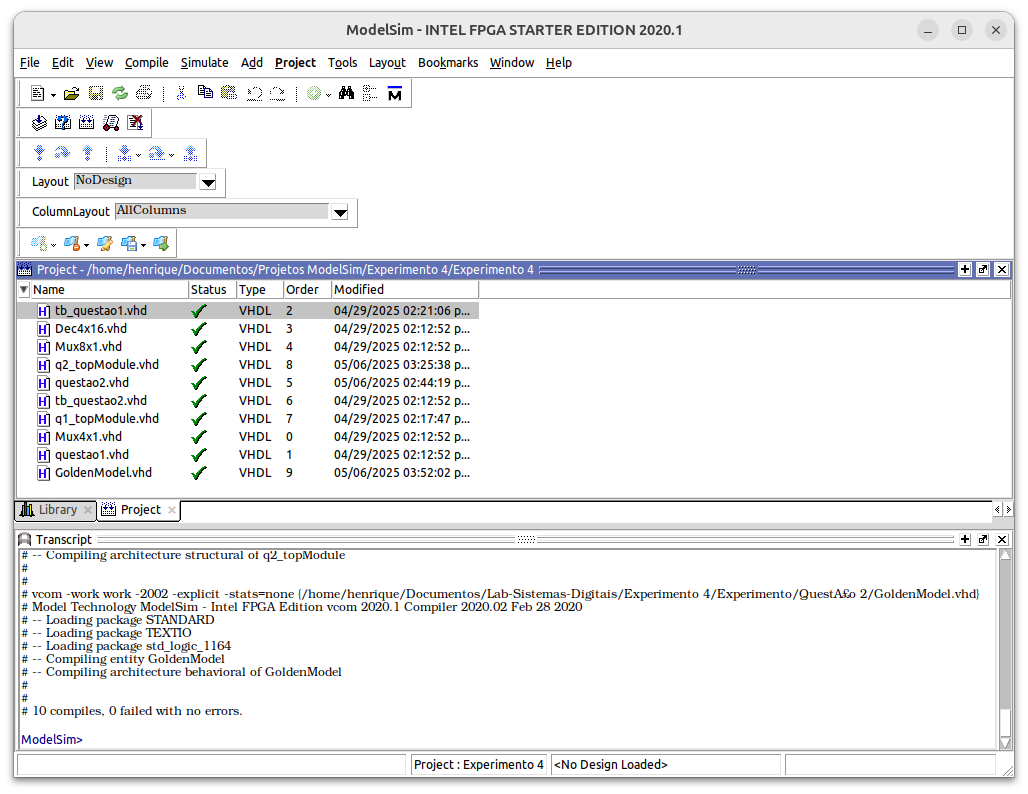
\includegraphics[width=1\textwidth]{Recursos/Imagens/CompileModelSim.png}
    \caption{Compilação de todos os códigos apresentados}
\end{figure}

\newpage

\section{Simulação}
As simulações do somador de \textit{nibble} e do seu \textit{Golden Model} estão exibidas a seguir. Os sinais de entrada estão em azul, a saída em verde e o \textit{Golden Model} em amarelo. O tempo de simulação para gerar todas as combinações é de $2^8\cdot 500ns = 128.000ns$.

\begin{figure}[H]
    \centering
    \begin{tcolorbox}[colframe=cinza, colback=white, boxrule=0.75pt, arc=0pt, width=1\textwidth, center, boxsep=0pt, left=0pt, right=0pt, top=0pt, bottom=0pt]
    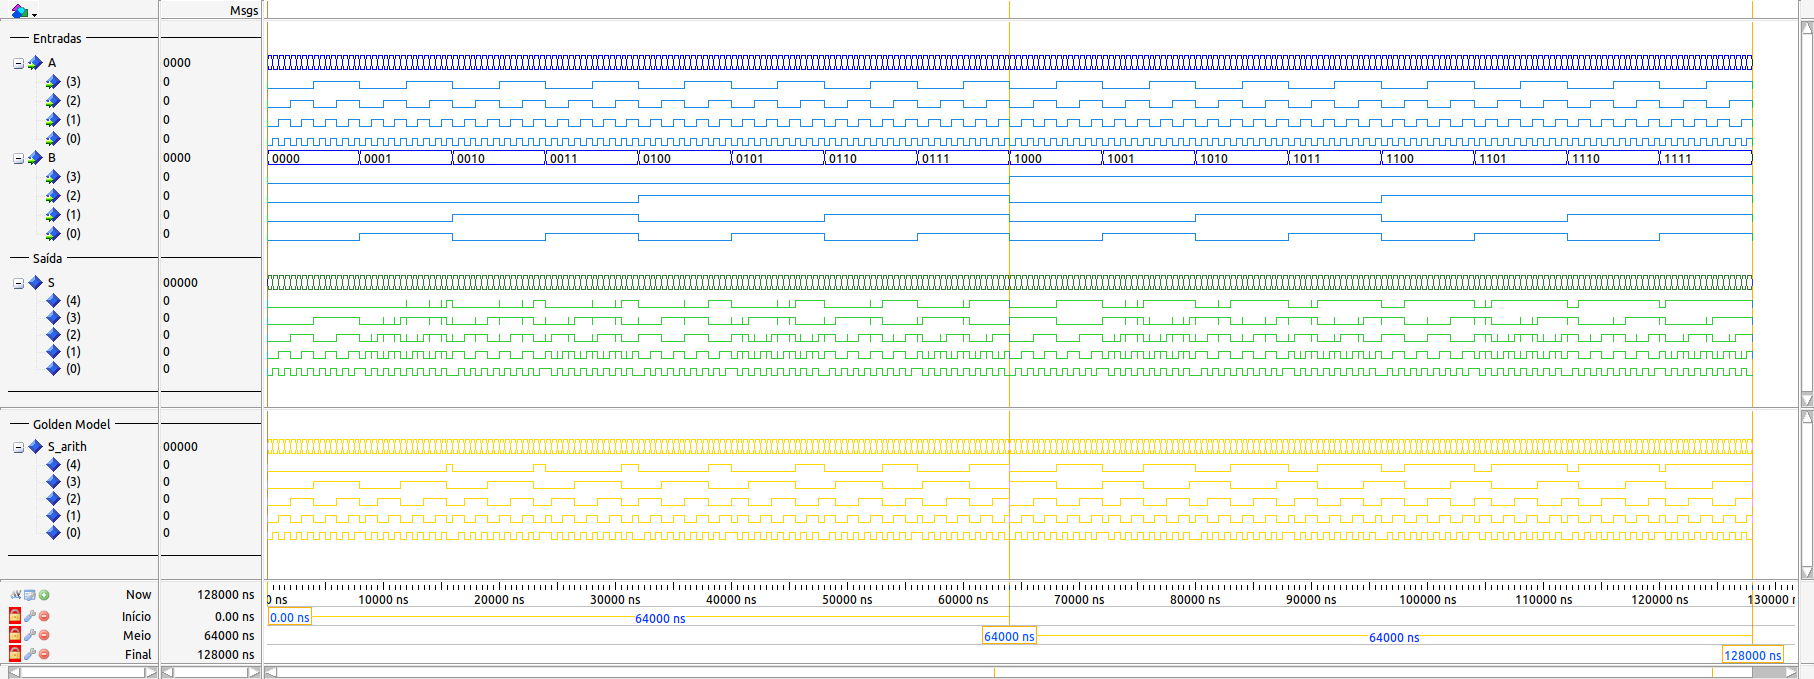
\includegraphics[width=1\textwidth]{Recursos/Imagens/SomadorNibble.png}
    \end{tcolorbox}
    \caption{Simulação em forma de onda binária do dispositivo da questão 1}
\end{figure}

Perceba que, na saída do somador de \textit{nibble} (não no \textit{Golden Model}), há oscilações de duração, aparentemente, infinitesimais. Não foi encontrada explicação para esse fenômeno e ele não ocorreu todas as vezes que o código foi simulado (quando foi recebido o visto, por exemplo). Ver-se-á doravante que essas variações não foram sequer reconhecidas pelo processo ``comparacoes'', mencionado anteriormente.

\newpage

\section{Análise}
A análise nesse experimento consiste em notar que as ondas do \textit{Golden Model} e do sistema testado são iguais, excetuando-se os picos e vales infinitesimais na saída do sistema. Isso é corroborado pela figura a seguir: notamos que no \textit{Transcript} (parte inferior da imagem) só foi exibida a mensagem de erro, definida no \textit{top module}, uma vez: no início da simulação, quando uma saída era ``UUUUU'' e a outra era ``XXXXX'' - caso limite, que não ilustra falha alguma na lógica de implementação utilizada.
\begin{figure}[H]
    \centering
    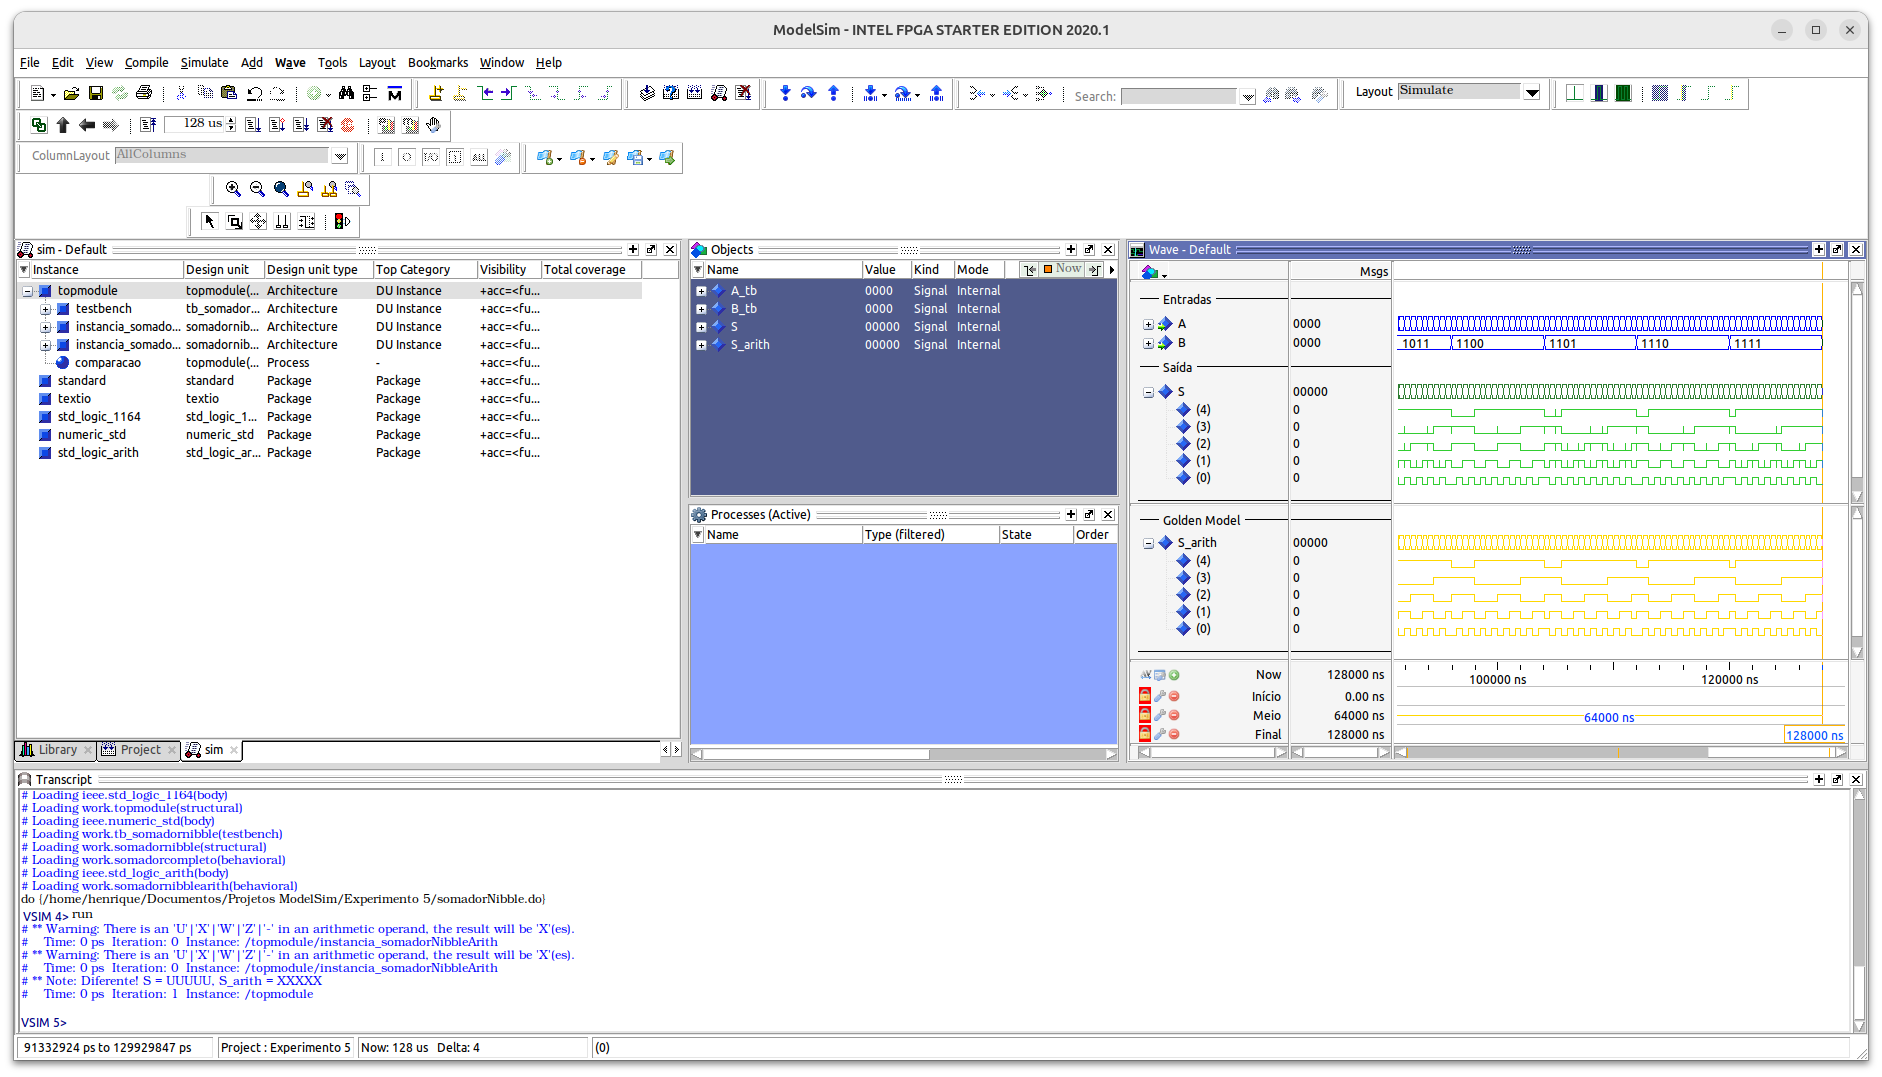
\includegraphics[width=1\linewidth]{Recursos/Imagens/Transcript.png}
    \caption{Tela do ModelSim após a simulação}
\end{figure}

\section{Conclusão}
Neste experimento, implementamos um somador de 4 \textit{bits} utilizando somadores completos, consolidando um conceito fundamental para a computação moderna, já que operações aritméticas como essa são a base do funcionamento da ULA (Unidade Lógica Aritmética) em processadores.

Além disso, ampliamos nosso conhecimento em metodologias de verificação com a introdução formal do \textit{Golden Model}, uma técnica essencial para validação de projetos digitais. Outro avanço significativo foi a utilização prática da biblioteca $std\_logic\_arith$ da Synopsys, que simplifica operações aritméticas em VHDL.

Por fim, o experimento não apenas reforçou conceitos-chave da disciplina, mas também demonstrou a importância de ferramentas automatizadas, como o \textit{Golden Model}, que eliminam a necessidade de verificações manuais exaustivas (como a comparação de todas as combinações de entradas), aumentando a eficiência e a confiabilidade do desenvolvimento.

\end{document}